\section{Mesons, wavefunctions and nomenclature}
\label{sec:mesons}

The previous chapter organized the light hadrons into the irreducible
representations of $\mathrm{SU(3)}_{F}$ and used the Gell-Mann--Okubo formula to
account for the mass splittings within the baryon multiplets. This chapter
specializes that machinery to the $q\bar q$ mesons. We first complete the catalogue
of meson quantum numbers begun in Sect.~\ref{sec:groups} by deriving the $G$ parity
and listing the accessible and the ``exotic'' $J^{PC}$ combinations. We then build
the meson nonet and analyze the symmetry of its wavefunctions in the combined
spin--flavor group $\mathrm{SU}(6)$, discuss the mixing of the two neutral
isoscalars and the special case of ideal mixing, fix the mixing angle from the meson
masses, and examine the dynamical consequences of the quark-line structure through
the Okubo--Zweig--Iizuka rule and the leptonic widths of the vector mesons. The
chapter closes with the modern naming scheme and with the $\eta$ meson as a precision
laboratory for the strong interaction and for physics beyond the Standard Model.

% ============================================================
\subsection{Quantum numbers and wavefunctions}
\label{subsec:qnumbers}

A meson is a bound quark--antiquark pair, the strong-interaction analogue of
positronium. Its internal wavefunction factorizes into a radial, an angular and a
spin part,
\begin{equation}
    \psi(\vec r,\vec s) = R(r)\,Y_{lm}(\theta,\phi)\,\chi(\vec s),
    \label{eq:meson_wavefunction}
\end{equation}
so that the total quark spin $S = s_q + s_{\bar q}$ takes the values $0$ or $1$ and
combines with the relative orbital angular momentum $L$ to give the meson spin
$J = L \oplus S$, with $|L-S| \le J \le L+S$. The state is conventionally labeled in
the spectroscopic notation $n^{\,2S+1}L_J$, where $n$ is the radial quantum number
and $L = S, P, D, \dots$ stands for $L = 0, 1, 2, \dots$
\cite[Ch.~2]{Amsler2018}. The parity and charge-conjugation eigenvalues of a
$q\bar q$ pair, derived in Sect.~\ref{sec:groups}, are
\begin{equation}
    P = (-1)^{L+1},
    \qquad
    C = (-1)^{L+s},
    \label{eq:meson_PC}
\end{equation}
the $C$ parity being defined only for the electrically neutral members with hidden
flavor ($S = C = B = 0$), for which the particle is its own antiparticle
\cite[Ch.~3]{Amsler2018}.

Charged mesons, and more generally any state with $I_{3} \neq 0$, cannot be eigenstates
of $C$ alone, since charge conjugation flips the sign of $I_{3}$ and therefore maps,
for instance, a $\pi^+$ onto a $\pi^-$,
\begin{equation}
    C\,\ket{\pi^+} = \eta_C\,\ket{\pi^-}.
\end{equation}
The eigenvalue can nevertheless be recovered by following the charge conjugation
with a rotation by $180^\circ$ about the $2$-axis in isospin space, represented by
the operator $R_U = \exp(i\pi I_2)$, which restores $I_{3}$ and hence the original
charge. The combined operation defines the \emph{$G$ parity}
\begin{equation}
    G = C\,e^{i\pi I_2},
    \label{eq:Gparity_def}
\end{equation}
of which the whole isospin multiplet is now a common eigenstate. For an isospin-$I$
multiplet the rotation contributes a factor $(-1)^I$, so that for a $q\bar q$ system
\begin{equation}
    G = C\,(-1)^I = (-1)^{L+s+I},
    \label{eq:Gparity}
\end{equation}
combining Eqs.~\eqref{eq:meson_PC} and \eqref{eq:Gparity_def}
\cite[Ch.~3]{Amsler2018}. Because both $C$ and isospin are conserved by the strong
interaction, $G$ parity is conserved as well; it is a practical bookkeeping device
rather than an independent symmetry. A particularly useful consequence is that a
system of $n$ pions has $G(n\pi) = (-1)^n$, which dictates that the $\rho$ ($G=+1$)
decays into two pions and the $\omega$ ($G=-1$) into three. The $G$ parity is not
defined for the $K$, $D$ and $B$ mesons, which carry open flavor
\cite[Ch.~3]{Amsler2018}.

% ------------------------------------------------------------
\subsubsection{Identical bosons in the final state}
\label{subsubsec:bose-symmetry}

The $G$-parity rule $G(n\pi) = (-1)^n$ is a necessary condition, not a sufficient one.
Whenever two or more of the final-state mesons are \emph{identical}, Bose symmetry
imposes a further restriction which forbids decays that $G$ parity alone would allow.
It is the exact counterpart of the Pauli argument used for the baryons in
Sect.~\ref{sec:baryons-color}: the total wavefunction of a system of identical bosons
must be \emph{symmetric} under their exchange.

For two identical pseudoscalars the wavefunction consists of a spatial part carrying
$(-1)^{L}$ and an isospin part. Exchange symmetry therefore requires the isospin
function to have the same symmetry as the spatial one. Coupling two $I=1$ pions gives
\begin{equation}
    \mathbf{3}\otimes\mathbf{3} = \mathbf{5}_S \oplus \mathbf{3}_A \oplus \mathbf{1}_S ,
    \label{eq:pipi_isospin}
\end{equation}
so $I = 2$ and $I = 0$ are symmetric while $I = 1$ is antisymmetric. A $\pi\pi$ state
therefore satisfies
\begin{equation}
    (-1)^{L} = (-1)^{I} \quad\Longrightarrow\quad L + I \;\text{even}.
    \label{eq:pipi_symmetry}
\end{equation}

Two consequences are used repeatedly. First, since a two-pion state has
$P = (-1)^{L}$ and, when neutral, $C = (-1)^{L}$, the combination $J^{PC} = 1^{--}$
requires $L = 1$ and hence, by Eq.~\eqref{eq:pipi_symmetry}, $I = 1$. The $\rho$ meson
duly decays to $\pi\pi$. Second---and this is the part $G$ parity does not capture---the
particular final state $\pi^0\pi^0$ consists of two \emph{identical} particles, for which
only the symmetric isospin combinations survive. The relevant Clebsch--Gordan coefficient
vanishes,
\begin{equation}
    \braket{1,0;1,0}{1,0} = 0 ,
    \label{eq:pi0pi0_CG}
\end{equation}
so a state of odd $L$ cannot decay into two neutral pions at all. Amsler reaches the
same conclusion from charge conjugation: for a pair of identical bosons $C$ permutes the
two particles, and Bose--Einstein symmetry then forces $L + s$ to be even, so that a
self-conjugate pair such as $\pi^0\pi^0$ or $\gamma\gamma$ is an eigenstate of $C$ with
eigenvalue $+1$ \cite[Ch.~3]{Amsler2018}. The same argument excludes spin $1$ for the
$\pi^0\pi^0$ system observed in $K_S$ decay \cite[Ch.~2]{Amsler2018}. Hence
\begin{equation*}
    \rho^0 \nrightarrow \pi^0\pi^0,
    \qquad
    \omega \nrightarrow \pi^0\pi^0 ,
\end{equation*}
even though $\rho^0 \to \pi^+\pi^-$ proceeds freely. Equivalently: two identical
pseudoscalars in a relative $L=1$ state would have to be antisymmetric in space and
symmetric in every other label, which Bose statistics forbids.

The same reasoning extends to three identical pions. The decay $\phi \to \pi^0\pi^0\pi^0$
is not forbidden by $G$ parity---$G(3\pi) = -1$ matches $G(\phi) = -1$---but it is
forbidden by the combination of $C$ parity and Bose symmetry. A system of three identical
neutral pions must be totally symmetric, and a totally symmetric $3\pi^0$ state cannot
carry the $J^{PC} = 1^{--}$ of the $\phi$. The observed decay is
$\phi \to \pi^+\pi^-\pi^0$, where the pions are not all identical and the constraint
relaxes. Arguments of exactly this kind are what fix the allowed initial states in
proton--antiproton annihilation (Sect.~\ref{subsec:annihilation}).

Equations~\eqref{eq:meson_PC} and \eqref{eq:Gparity} restrict the quantum numbers
that a simple $q\bar q$ pair can carry. Running through the lowest values of $L$ and
$S$ gives the accessible combinations
\begin{equation}
    J^{PC}(q\bar q) = 0^{-+},\,0^{++},\,1^{--},\,1^{+-},\,1^{++},\,
                      2^{--},\,2^{-+},\,2^{++},\,3^{--},\,3^{+-},\,3^{++},\,\dots
    \label{eq:allowed_JPC}
\end{equation}
while the values
\begin{equation}
    J^{PC} = 0^{--},\,0^{+-},\,1^{-+},\,2^{+-},\,3^{-+},\,\dots
    \label{eq:exotic_JPC}
\end{equation}
cannot be reached by any $L,S$ assignment. A state observed with one of these
\emph{exotic} quantum numbers cannot be a conventional meson and must instead be a
glueball ($gg$), a hybrid ($q\bar q g$), a meson--meson molecule, or a multiquark
state such as a tetraquark ($q\bar q q\bar q$); these configurations are taken up in
a later chapter \cite[Ch.~4]{Amsler2018}. The catalogue \eqref{eq:exotic_JPC}
thereby turns the elementary counting of $q\bar q$ quantum numbers into an
experimental search strategy for physics beyond the naive quark model.

\begin{figure}[htbp]
    \centering
    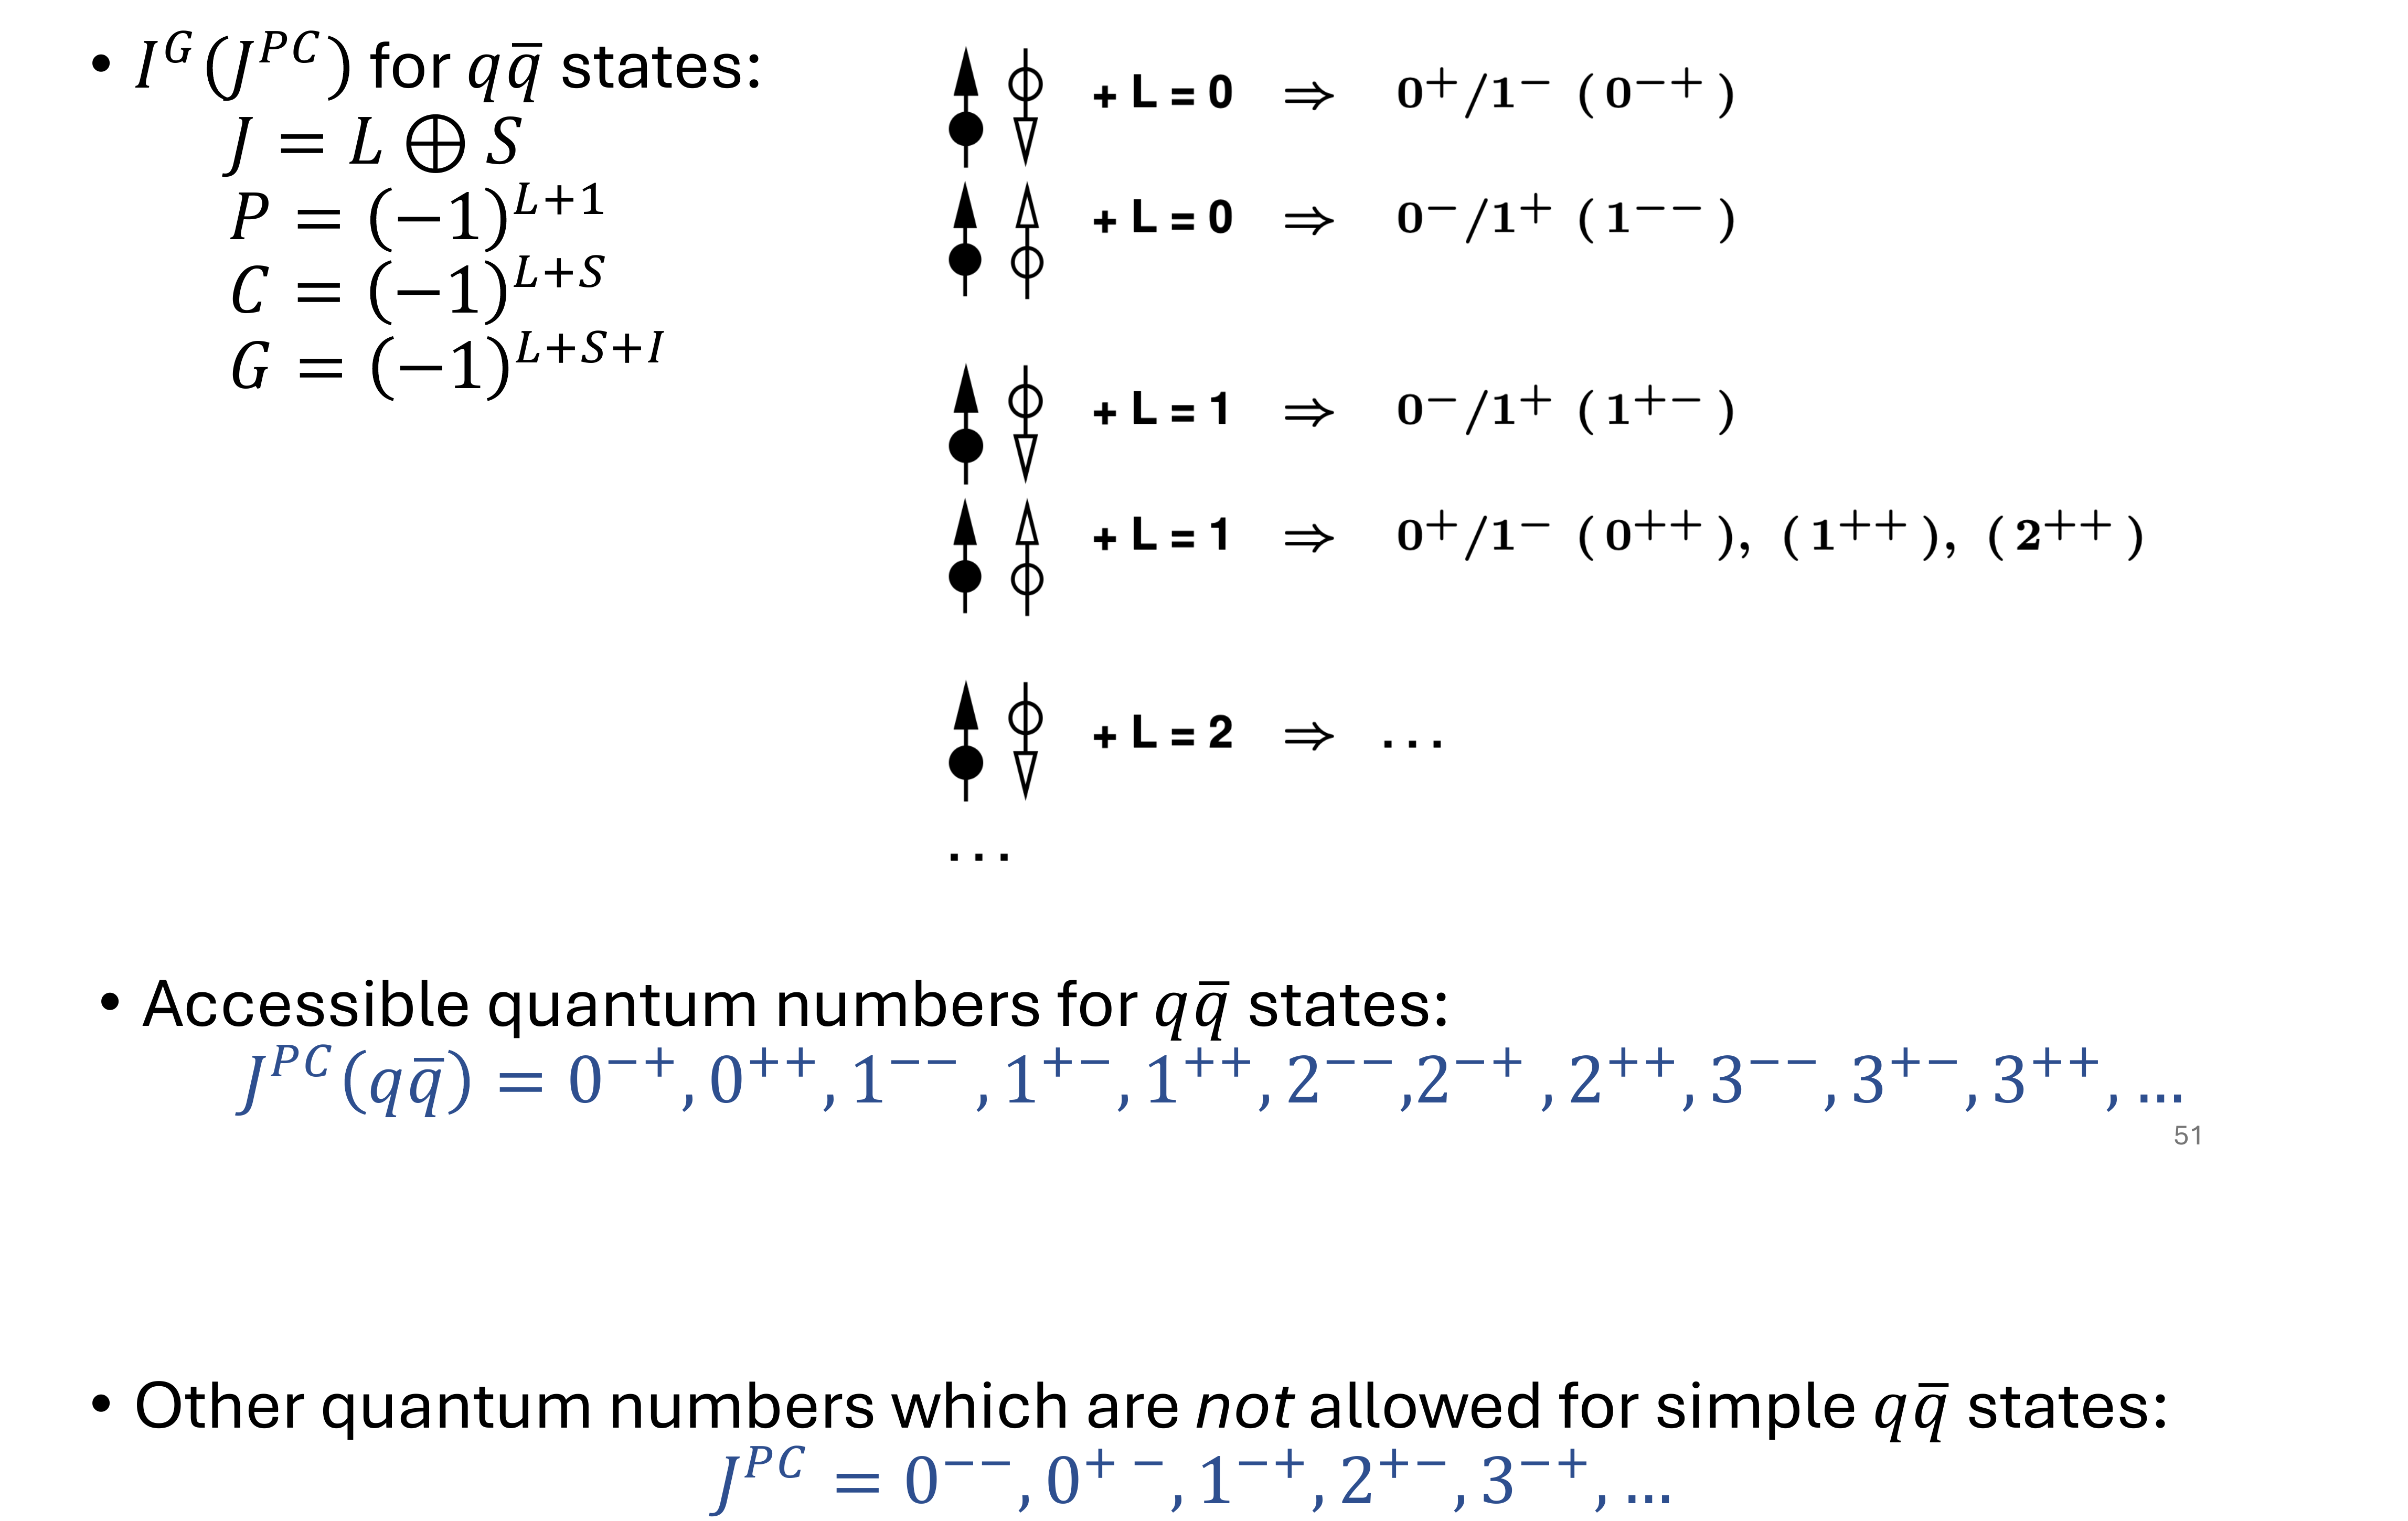
\includegraphics[width=0.85\linewidth]{Figures/qqbar_JPC_ladder.png}
    \caption{Spin and orbital angular momentum of a $q\bar q$ pair and the
    resulting $J^{PC}$ quantum numbers. The combinations
    in the lower block (Eq.~\eqref{eq:exotic_JPC}) cannot be formed by a simple
    quark--antiquark pair and are termed exotic. Adapted from the lecture
    slides (week 19, "Possible quantum numbers of $q\bar q$ states").}
    \label{fig:jpc_ladder}
\end{figure}

% ============================================================
\subsection{Mesons}
\label{subsec:mesons}

With three flavors of light quark the fundamental representation of
$\mathrm{SU(3)}_{F}$ is the triplet $(u,d,s)$, and a $q\bar q$ pair lives in the product
\begin{equation}
    \mathbf{3}\otimes\overline{\mathbf{3}} = \mathbf{1}\oplus\mathbf{8},
    \label{eq:nonet_decomp}
\end{equation}
so that, for a given $J^{PC}$, the nine quark--antiquark combinations group into an
octet and a singlet---the meson \emph{nonet} \cite[Ch.~7]{Amsler2018}. The six
states on the periphery of the weight diagram carry open flavor and are uniquely
fixed; for the pseudoscalars they are the kaons $K^+ = u\bar s$, $K^0 = d\bar s$,
$\bar K^0 = s\bar d$, $K^- = s\bar u$ together with the charged pions
$\pi^+ = u\bar d$ and $\pi^- = d\bar u$. The three states sitting at the center of
the hexagon all have $I_{3} = Y = 0$ and must be disentangled. The neutral member of
the isotriplet cannot contain an $s\bar s$ component and is
\begin{equation}
    \ket{8,3} = \tfrac{1}{\sqrt 2}\,\ket{u\bar u - d\bar d}
    \;\;(\,\widehat{=}\;\pi^0\;\text{or}\;\rho^0\,),
    \label{eq:pi0_state}
\end{equation}
while the two isoscalars are the $\mathrm{SU}(3)$ singlet and the isoscalar member of
the octet, obtained by Gram--Schmidt orthogonalisation,
\begin{align}
    \ket{1,1} &= \tfrac{1}{\sqrt 3}\,\ket{u\bar u + d\bar d + s\bar s}, \\
    \ket{8,1} &= \tfrac{1}{\sqrt 6}\,\ket{u\bar u + d\bar d - 2s\bar s},
    \label{eq:singlet_octet}
\end{align}
the singlet being the flavor-symmetric, $\mathrm{SU}(3)$-invariant combination and
the octet state the one orthogonal both to it and to Eq.~\eqref{eq:pi0_state}
\cite[Ch.~7]{Amsler2018}.

The permutation symmetry of the meson wavefunction is most transparent in the
combined spin--flavor group obtained by merging the flavor group
$\mathrm{SU(3)}_{F}$ with the spin group $\mathrm{SU}(2)_{\text{spin}}$ into
$\mathrm{SU}(6)$, whose fundamental representation contains the six states
$u\!\uparrow, d\!\uparrow, s\!\uparrow, u\!\downarrow, d\!\downarrow, s\!\downarrow$.
A meson wavefunction factorizes as
\begin{equation}
    \psi = \Phi_{\text{flavor}}\,\chi_{\text{spin}}\,\lambda_{\text{color}}\,R(\vec{r}\,),
    \label{eq:su6_wavefunction}
\end{equation}
where the color part $\lambda_{\text{color}}$ is the $q\bar q$ singlet. It is
totally symmetric and carries no free index, so it plays no role in the symmetry
counting below and is suppressed from here on.
and since the flavor part decomposes according to Eq.~\eqref{eq:nonet_decomp} into
symmetric and antisymmetric combinations $\Phi_S, \Phi_A$, while the two spins
combine into symmetric ($\chi_S$, $s=1$) and antisymmetric ($\chi_A$, $s=0$) parts,
there are four possible products: the symmetric $\Phi_S\chi_S$ and $\Phi_A\chi_A$,
and the antisymmetric $\Phi_S\chi_A$ and $\Phi_A\chi_S$
\cite[Ch.~7]{Amsler2018}. The physically realized symmetry is fixed by charge
conjugation, which exchanges quark and antiquark and acts on the flavor part with
the factor $(-1)^{L+s}$ of Eq.~\eqref{eq:meson_PC}. For the pseudoscalar ground
states ($L = s = 0$, spin function $\chi_A$),
\begin{equation}
    C\ket{\pi^0} = C(\Phi\chi) = (-1)^{0+0}\,\Phi\chi = +\Phi\chi = \Phi_S\chi
    \;\;\Longrightarrow\;\; \psi(\pi^0) = \Phi_S\chi_A,
\end{equation}
which is overall antisymmetric, while for the vector ground states ($L=0$, $s=1$,
spin function $\chi_S$),
\begin{equation}
    C\ket{\rho^0} = (-1)^{0+1}\,\Phi\chi = -\Phi\chi = \Phi_A\chi
    \;\;\Longrightarrow\;\; \psi(\rho^0) = \Phi_A\chi_S,
\end{equation}
again antisymmetric overall. Consistently, the neutral isovector
Eq.~\eqref{eq:pi0_state} is realized as the flavor-symmetric combination for the
pseudoscalar and as the flavor-antisymmetric combination for the vector
\cite[Ch.~7]{Amsler2018}.

\begin{figure}[htbp]
    \centering
    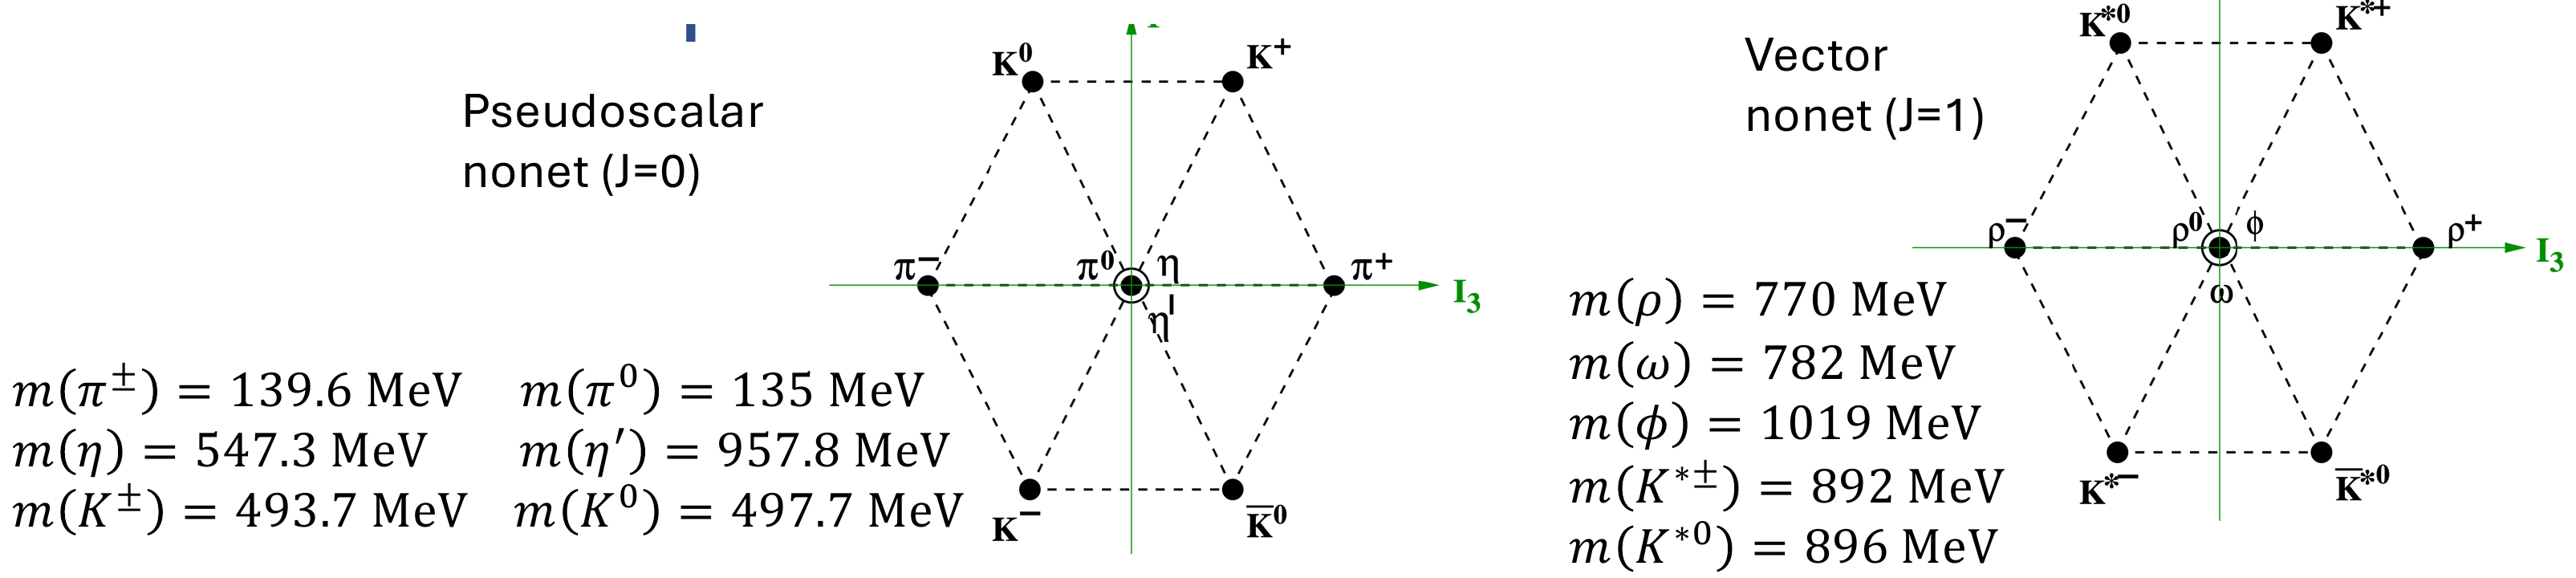
\includegraphics[width=0.9\linewidth]{Figures/meson_nonets.png}
    \caption{Weight diagrams of the pseudoscalar ($J^{PC} = 0^{-+}$) and vector
    ($J^{PC} = 1^{--}$) meson nonets in the $(I_3, Y)$ plane. The six
    open-flavor states lie on the periphery of the hexagon; the three neutral,
    flavorless states occupy the center. Adapted from the lecture slides
    (week 19, "Meson multiplets").}
    \label{fig:meson_nonets}
\end{figure}

% ============================================================
\subsection{Nonets and ideal mixing}
\label{subsec:nonets}

The two central isoscalars $\ket{8,1}$ and $\ket{1,1}$ share all conserved quantum
numbers ($Q = I = S = 0$) and therefore mix. The physically observed states are the
orthogonal superpositions
\begin{align}
    \ket{f_A} &= \cos\theta\,\ket{8,1} - \sin\theta\,\ket{1,1}, \notag\\
    \ket{f_B} &= \sin\theta\,\ket{8,1} + \cos\theta\,\ket{1,1},
    \label{eq:nonet_mixing}
\end{align}
with a single mixing angle $\theta$ that must be determined from experiment by
comparing masses, decays and production properties \cite[Ch.~5]{Amsler2018}. A
distinguished value is \emph{ideal mixing},
\begin{equation}
    \tan\theta = \frac{1}{\sqrt 2}
    \;\;\Longleftrightarrow\;\;
    \theta = 35.3^\circ,
    \label{eq:ideal_mixing}
\end{equation}
for which the $s\bar s$ component decouples completely from the light quarks, so that
one physical isoscalar becomes pure strange and the other a pure $u,d$ combination,
\begin{equation}
    \ket{f_A} = -\ket{s\bar s},
    \qquad
    \ket{f_B} = \tfrac{1}{\sqrt 2}\,\ket{u\bar u + d\bar d}.
    \label{eq:ideal_states}
\end{equation}

The vector nonet is very close to ideal mixing. The near degeneracy
$m(\rho(770)) \approx m(\omega(782))$ already signals that the $\omega$ shares the
light-quark content of the $\rho^0$, and the assignment
$\ket{\omega} = \tfrac{1}{\sqrt 2}\ket{u\bar u + d\bar d}$,
$\ket{\phi} = -\ket{s\bar s}$ follows with $\theta_V \approx 35.3^\circ$
\cite[Ch.~5]{Amsler2018}. The pseudoscalar nonet is the conspicuous exception: its
mixing angle lies in the range $-10^\circ$ to $-20^\circ$, far from ideal, so that
the $\eta$ and $\eta'$ are close to the pure octet and singlet states of
Eq.~\eqref{eq:singlet_octet}. The reason is dynamical. The mixing is driven by the
annihilation of the $q\bar q$ pair into intermediate gluons; for the $0^{-+}$
isoscalars a two-gluon intermediate state is allowed, generating a large
perturbation, whereas for the $1^{--}$ isoscalars the Landau--Yang theorem forbids a
spin-$1$ state from coupling to two massless spin-$1$ gluons, so at least three gluons are
required and the perturbation is strongly suppressed \cite[Ch.~5]{Amsler2018}.%
\footnote{Amsler calls this the ``Fermi--Yang theorem'' at this point in Sect.~5.2,
but cites Landau (1948) and Yang (1950) as the reference and uses the standard name
Landau--Yang everywhere else, including the proof in his Appendix~A. The Fermi--Yang
model is the unrelated 1949 proposal of the pion as an $N\bar N$ bound state.} This
is why the vectors mix ideally while the pseudoscalars do not. The measured masses
of the two ground-state nonets,
\begin{equation}
\begin{aligned}
    &m(\pi^\pm) = 139.6,\;\; m(\pi^0) = 135,\;\;
     m(\eta) = 547.3,\;\; m(\eta') = 957.8,\\
    &m(K^\pm) = 493.7,\;\; m(K^0) = 497.7
    \qquad\text{(pseudoscalars)},\\[2pt]
    &m(\rho) = 770,\;\; m(\omega) = 782,\;\; m(\phi) = 1019,\;\;
     m(K^{*\pm}) = 892,\;\; m(K^{*0}) = 896
     \quad\text{(vectors)},
\end{aligned}
\label{eq:nonet_masses}
\end{equation}
(in MeV) are the inputs to the mass formulae of the next subsection
\cite[Ch.~5]{Amsler2018}.

\begin{figure}[htbp]
    \centering
    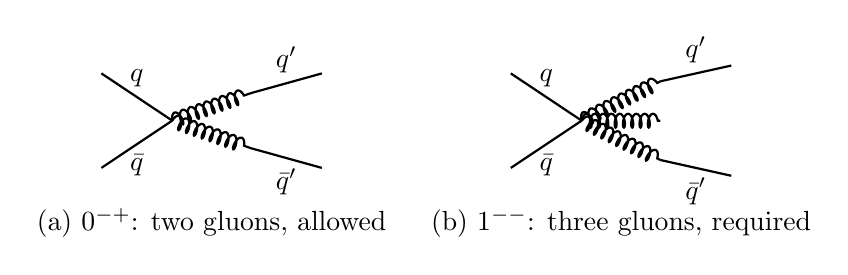
\begin{tikzpicture}[thick, scale=1.0]
        % Left: 2-gluon process (pseudoscalar, allowed)
        \begin{scope}
            \draw (-1.4,0.6) -- (-0.5,0) node[midway, above] {$q$};
            \draw (-1.4,-0.6) -- (-0.5,0) node[midway, below] {$\bar q$};
            \draw[decorate,decoration={coil,aspect=0.4,segment length=3pt}]
                (-0.5,0) -- (0.5,0.35);
            \draw[decorate,decoration={coil,aspect=0.4,segment length=3pt}]
                (-0.5,0) -- (0.5,-0.35);
            \draw (0.5,0.35) -- (1.4,0.6) node[midway, above] {$q'$};
            \draw (0.5,-0.35) -- (1.4,-0.6) node[midway, below] {$\bar q'$};
            \node at (0,-1.3) {(a) $0^{-+}$: two gluons, allowed};
        \end{scope}
        % Right: 3-gluon process (vector, required)
        \begin{scope}[xshift=5.2cm]
            \draw (-1.4,0.6) -- (-0.5,0) node[midway, above] {$q$};
            \draw (-1.4,-0.6) -- (-0.5,0) node[midway, below] {$\bar q$};
            \draw[decorate,decoration={coil,aspect=0.4,segment length=3pt}]
                (-0.5,0) -- (0.5,0.5);
            \draw[decorate,decoration={coil,aspect=0.4,segment length=3pt}]
                (-0.5,0) -- (0.5,0);
            \draw[decorate,decoration={coil,aspect=0.4,segment length=3pt}]
                (-0.5,0) -- (0.5,-0.5);
            \draw (0.5,0.5) -- (1.4,0.7) node[midway, above] {$q'$};
            \draw (0.5,-0.5) -- (1.4,-0.7) node[midway, below] {$\bar q'$};
            \node at (0,-1.3) {(b) $1^{--}$: three gluons, required};
        \end{scope}
    \end{tikzpicture}
    \caption{Gluonic perturbation responsible for singlet--octet mixing. (a)
    The pseudoscalar ($0^{-+}$) isoscalars can mix via an intermediate
    two-gluon state. (b) The Landau--Yang theorem forbids a spin-$1$ state from
    coupling to two massless spin-$1$ gluons, so the vector ($1^{--}$) isoscalars
    require at least three gluons, strongly suppressing the perturbation;
    this explains the near-ideal mixing of the vector nonet and the large
    deviation of the pseudoscalars.}
    \label{fig:mixing_perturbation}
\end{figure}

% ============================================================
\subsection{The Gell-Mann--Okubo mass formula}
\label{subsec:gmo-mesons}

The mass formula introduced for the baryon multiplets in
Sect.~\ref{subsec:gmo} applies equally to the mesons, with the mixing angle now
following from the nonet masses. Treating the quark masses additively, the
pseudoscalar masses are
\begin{equation}
    M_\pi = M_0 + 2M_q,
    \qquad
    M_K = M_0 + M_q + M_s,
    \label{eq:gmo_piK}
\end{equation}
while the pure octet and singlet states carry
\begin{equation}
    M_8 = M_0 + \tfrac{2}{3}M_q + \tfrac{4}{3}M_s,
    \qquad
    M_1 = M_0 + \tfrac{4}{3}M_q + \tfrac{2}{3}M_s,
    \label{eq:gmo_18}
\end{equation}
corresponding to the octet and singlet wavefunctions of
Eq.~\eqref{eq:singlet_octet}. Eliminating the unknown quark masses yields the two
relations
\begin{equation}
    4M_K - M_\pi = 3M_8,
    \qquad
    2M_K + M_\pi = 3M_1.
    \label{eq:gmo_relations}
\end{equation}
Diagonalising the $2\times2$ mass matrix in the basis $(\ket{8,1}, \ket{1,1})$ and
identifying the eigenvalues with the physical $\eta$ and $\eta'$ masses through
$\langle\varphi|H|\varphi\rangle = M_\varphi$ gives, with the off-diagonal element
$M_{18} = \langle 8,1|H|1,1\rangle$,
\begin{align}
    M_\eta   &= M_8\cos^2\theta + M_1\sin^2\theta - 2M_{18}\sin\theta\cos\theta,
    \notag\\
    M_{\eta'} &= M_8\sin^2\theta + M_1\cos^2\theta + 2M_{18}\sin\theta\cos\theta,
    \notag\\
    0 &= (M_8 - M_1)\sin\theta\cos\theta + M_{18}(\cos^2\theta - \sin^2\theta),
    \label{eq:gmo_matrix}
\end{align}
the last line expressing the vanishing of the off-diagonal element in the physical
basis. Solving for the angle yields the \emph{linear mass formula}
\begin{equation}
    \tan^2\theta =
    \frac{3M_\eta + M_\pi - 4M_K}{4M_K - 3M_{\eta'} - M_\pi},
    \label{eq:gmo_linear}
\end{equation}
which has an often-used variant, the \emph{quadratic mass formula}, obtained by
replacing each mass by its square,
\begin{equation}
    \tan^2\theta =
    \frac{3M_\eta^2 + M_\pi^2 - 4M_K^2}{4M_K^2 - 3M_{\eta'}^2 - M_\pi^2}.
    \label{eq:gmo_quadratic}
\end{equation}
There is no compelling theoretical reason to prefer one over the other, and the two
return appreciably different angles \cite[Ch.~5]{Amsler2018}. Applied to the
established nonets the formulae give the values collected in
Table~\ref{tab:mixing_angles}; the vector nonet comes out closest to the ideal
$35.3^\circ$, the tensor and $3^{--}$ nonets sit somewhat below it near
$28$--$32^\circ$, while the pseudoscalars are small and negative, consistent
with the dynamical argument of Sect.~\ref{subsec:nonets}.

\begin{table}[t]
    \centering
    \caption{Mixing angles $\Theta$ extracted from the linear
    (Eq.~\eqref{eq:gmo_linear}) and quadratic (Eq.~\eqref{eq:gmo_quadratic}) mass
    formulae for the well-established meson nonets \cite[Ch.~5]{Amsler2018}.}
    \label{tab:mixing_angles}
    \begin{tabular}{lcc}
        \hline
        Nonet members &
        $\Theta_{\mathrm{linear}}$ &
        $\Theta_{\mathrm{quad}}$ \\
        \hline
        $\pi,\,K,\,\eta',\,\eta$ &
        $-24.5^\circ$ & $-11.3^\circ$ \\
        $\rho(770),\,K^*(892),\,\phi(1020),\,\omega(783)$ &
        $36.5^\circ$ & $39.2^\circ$ \\
        $a_2(1320),\,K_2^*(1430),\,f_2'(1525),\,f_2(1270)$ &
        $28.0^\circ$ & $29.6^\circ$ \\
        $\omega_3(1670),\,K_3^*(1780),\,\phi_3(1850),\,\rho_3(1690)$ &
        $30.8^\circ$ & $31.8^\circ$ \\
        \hline
    \end{tabular}
\end{table}

For the pseudoscalars the small angle $\theta \approx -19.3^\circ$ leads to the
explicit wavefunctions
\begin{equation}
    \ket{\eta}  = \tfrac{1}{\sqrt 3}\,\ket{u\bar u + d\bar d - s\bar s},
    \qquad
    \ket{\eta'} = \tfrac{1}{\sqrt 6}\,\ket{u\bar u + d\bar d + 2s\bar s},
    \label{eq:eta_states}
\end{equation}
which interpolate between the pure octet/singlet limit ($\theta = 0^\circ$) and the
ideally mixed case ($\theta = 35.3^\circ$), where $\ket{f_A} = -\ket{s\bar s}$
\cite[Ch.~5]{Amsler2018}. The same relations applied to the baryon multiplets were
discussed in Sect.~\ref{subsec:gmo}.

% ============================================================
\subsection{The OZI rule}
\label{subsec:ozi}

The Okubo--Zweig--Iizuka (OZI) rule states that a strong decay whose Feynman graph
can be separated into the initial and final hadrons \emph{without cutting any quark
line} is suppressed: the process may still proceed, but with a probability
comparable to that of an electromagnetic transition \cite[Ch.~5]{Amsler2018}.
Intuitively, the decay rate diminishes the more $q\bar q$ pairs have to be created
out of the vacuum. The textbook illustration is the $\phi(1020)$, which is almost
pure $s\bar s$. Its decay into $K\bar K$ proceeds through connected quark lines and is
OZI allowed, whereas the decay into $\pi^+\pi^-\pi^0$ requires the initial $s$ and
$\bar s$ to annihilate and three new light pairs to be produced, a disconnected
graph that is OZI suppressed. The suppression survives despite the very different
phase space available, the $Q$ value being about $600$~MeV for $3\pi$ but only about
$20$~MeV for $K\bar K$. The branching ratios bear this out, with
$BR(\phi\to K\bar K)\approx 84\%$ against $BR(\phi\to 3\pi)\approx 15\%$, and the
narrow total width $\Gamma(\phi) = 4.4$~MeV contrasts sharply with the
OZI-unsuppressed $\Gamma(\rho(770)) = 150$~MeV \cite[Ch.~5]{Amsler2018}.

\begin{figure}[htbp]
    \centering
    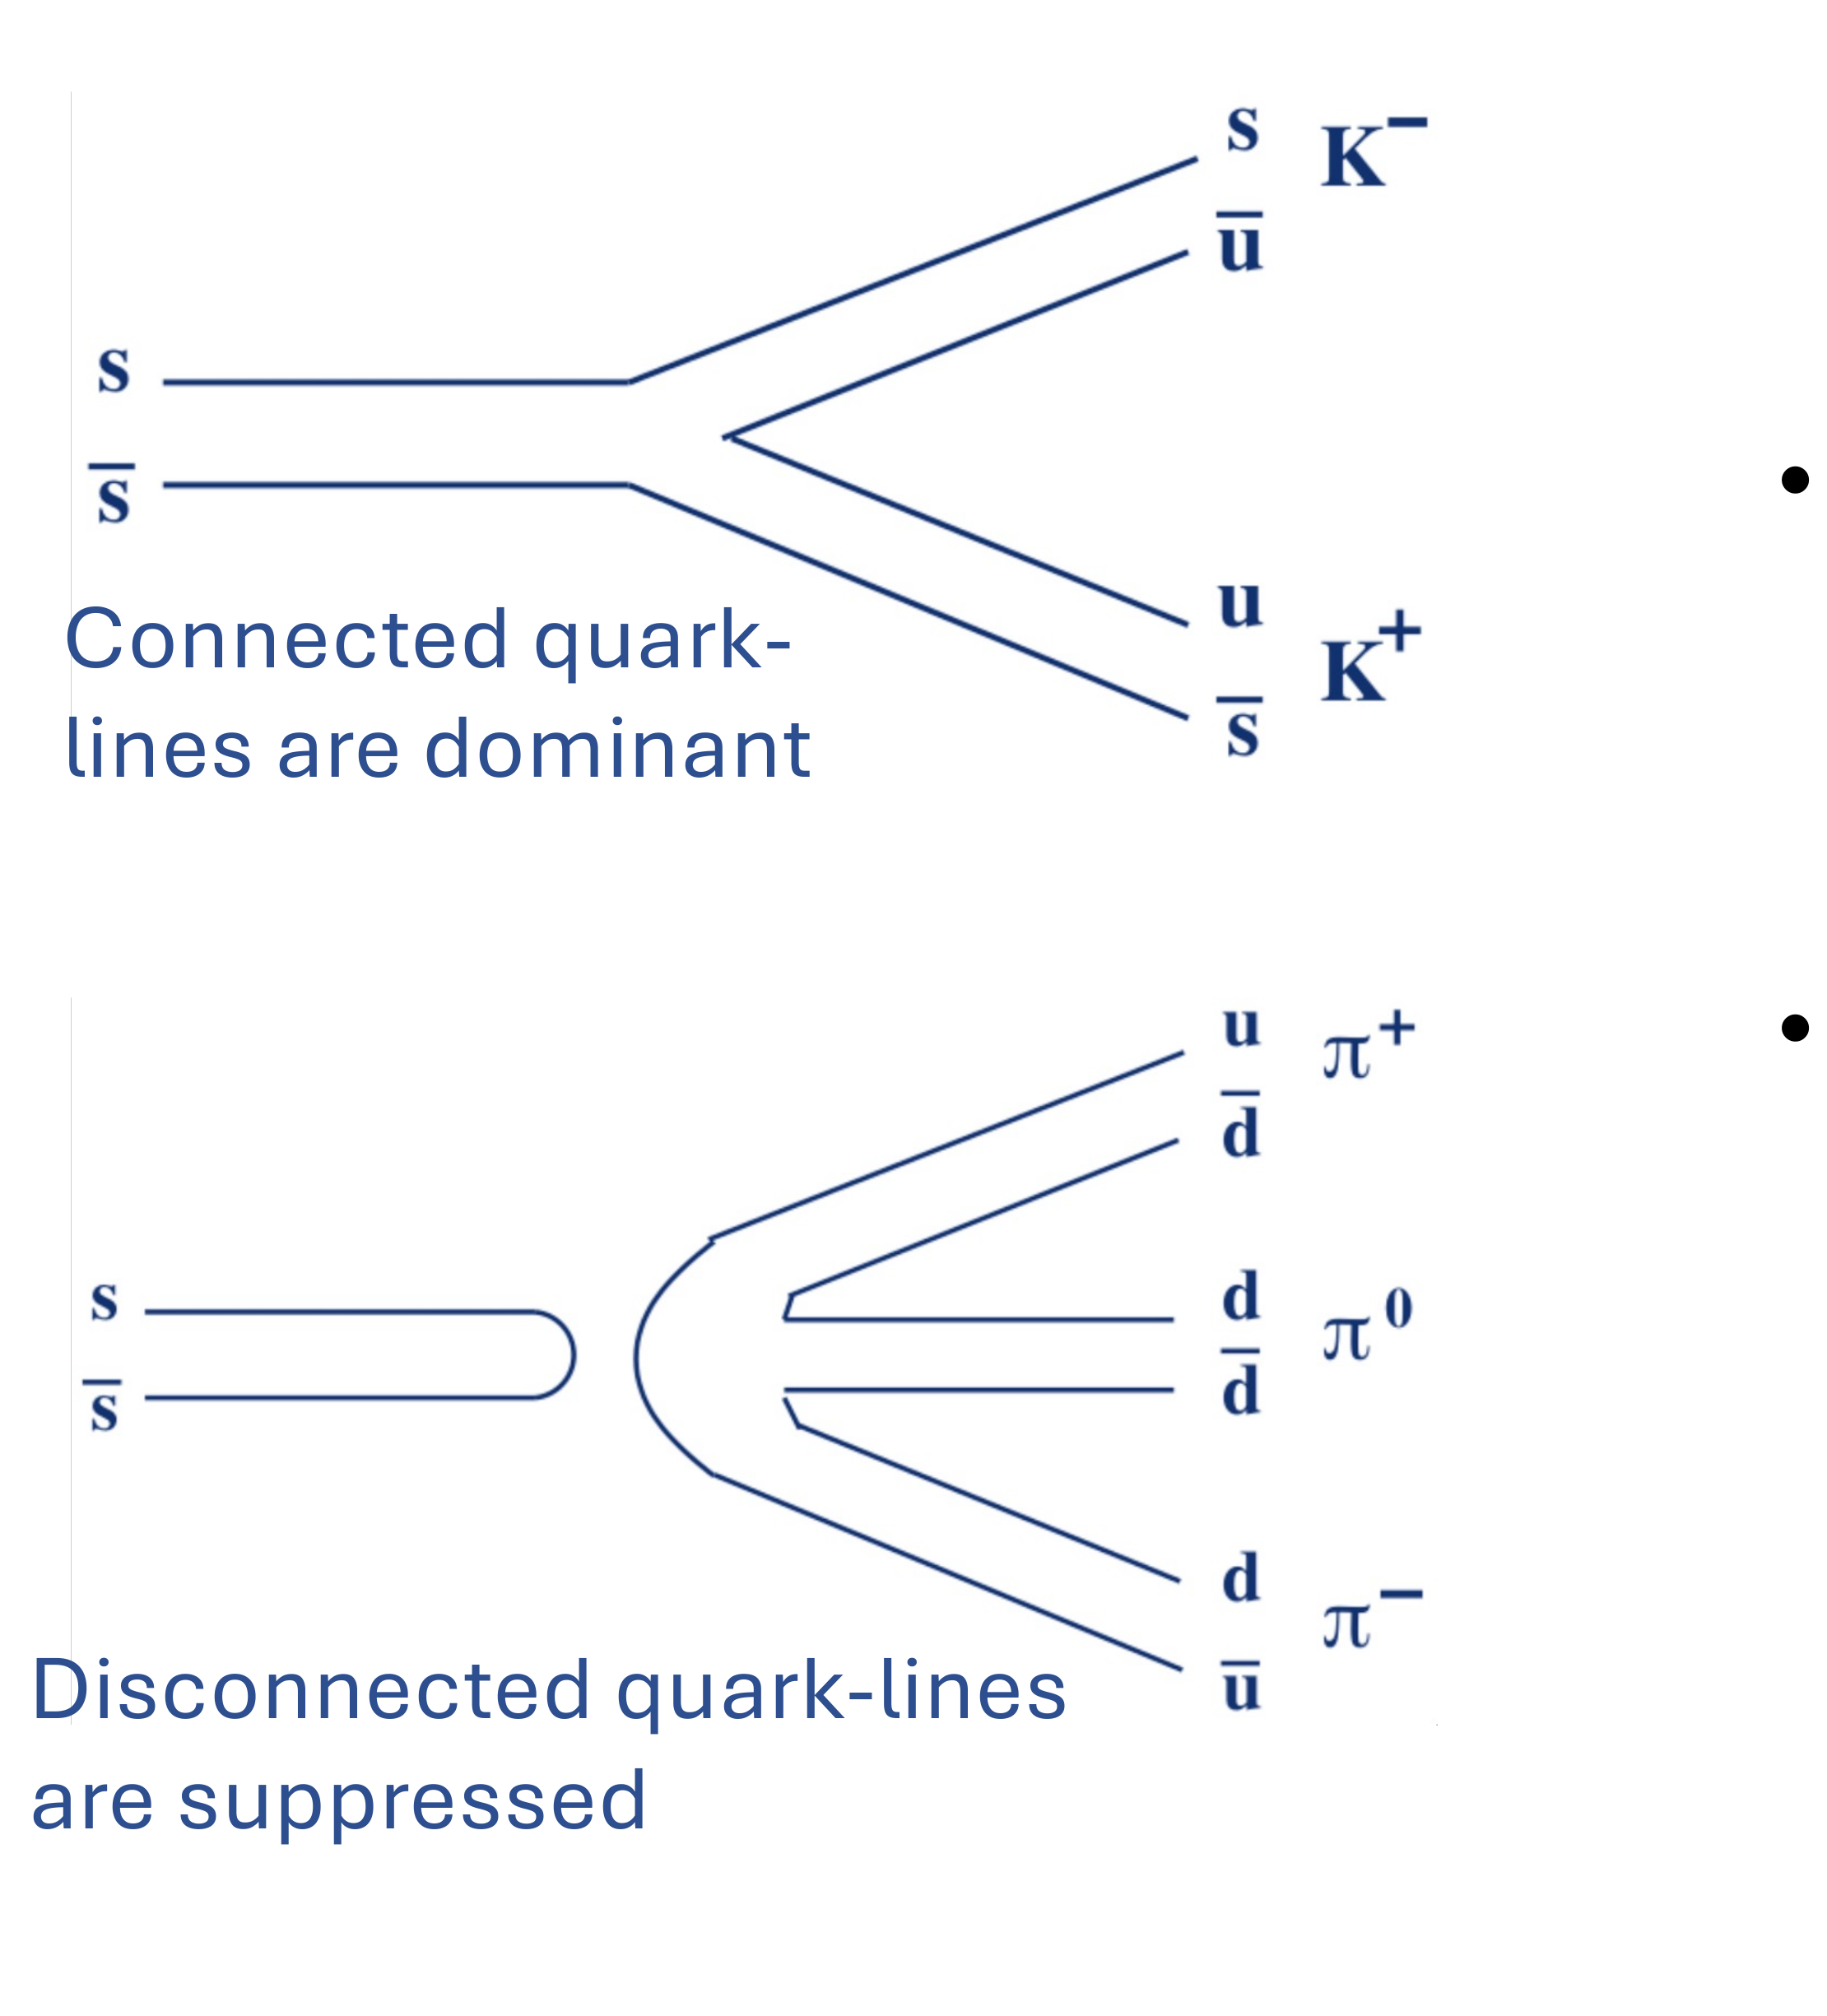
\includegraphics[width=0.55\linewidth]{Figures/ozi_phi.png}
    \caption{Quark-line diagrams for $\phi(s\bar s)$ decay. The connected
    $K\bar K$ graph (top) is OZI allowed and dominates, whereas the
    disconnected $3\pi$ graph (bottom), in which the $s\bar s$ pair
    annihilates, is OZI suppressed. Adapted from the lecture slides (week 19,
    "OZI rule").}
    \label{fig:ozi_phi}
\end{figure}

A complementary and more quantitative probe of the quark content is the leptonic
width of the vector mesons, the decay $V \to e^+e^-$ proceeding through a single
virtual photon coupling to the quark charges. The rate is proportional to the square
of the charge-weighted sum of the flavor amplitudes,
\begin{equation}
    \Gamma(V \to e^+e^-) \;\propto\; \Big|\textstyle\sum_q e_q\,c_q\Big|^2,
    \label{eq:leptonic_width}
\end{equation}
where $e_q$ are the quark charges and $c_q$ the wavefunction coefficients. Inserting
the ideally mixed states $\ket{\rho^0} = \tfrac{1}{\sqrt 2}\ket{u\bar u - d\bar d}$,
$\ket{\omega} = \tfrac{1}{\sqrt 2}\ket{u\bar u + d\bar d}$ and
$\ket{\phi} = -\ket{s\bar s}$ with $e_u = +\tfrac{2}{3}$,
$e_d = e_s = -\tfrac{1}{3}$ gives the squared amplitudes $\tfrac12$, $\tfrac{1}{18}$
and $\tfrac19$, that is
\begin{equation}
    \Gamma_\rho : \Gamma_\omega : \Gamma_\phi = 9 : 1 : 2.
    \label{eq:leptonic_ratio}
\end{equation}
The measured widths in Table~\ref{tab:leptonic_widths} reproduce the predicted
hierarchy remarkably well given the crudeness of the single-photon estimate
\cite[Ch.~7]{Amsler2018}. The residual discrepancies, most visibly for the $\rho^0$,
arise from $\rho$--$\omega$ interference: the small $u$--$d$ mass difference breaks
charge symmetry so that the physical $\rho$ and $\omega$ are not pure isospin
eigenstates but each contain a small admixture of the other's isospin, an effect
studied for instance by the Crystal Barrel collaboration in $\bar p p$ annihilation.

\begin{table}[t]
    \centering
    \caption{Leptonic widths $\Gamma_{e^+e^-}$ of the vector mesons compared with
    the quark-charge prediction of Eq.~\eqref{eq:leptonic_width}. Experimental
    values from the PDG; the ratios are normalized to the $\omega$
    \cite[Ch.~7]{Amsler2018}.}
    \label{tab:leptonic_widths}
    \begin{tabular}{lccccc}
        \hline
         & $\rho^0$ & $\omega$ & $\phi$ & $J/\psi$ & $\Upsilon$ \\
        \hline
        $\Gamma_{e^+e^-}$ [keV] &
        $7.04$ & $0.60$ & $1.27$ & $5.53$ & $1.34$ \\
        Measured ratio &
        $\sim\!11.7$ & $\sim\!1$ & $\sim\!2.1$ & $\sim\!9.2$ & $\sim\!2.2$ \\
        Expected ratio &
        $\sim\!9$ & $\sim\!1$ & $\sim\!2$ & $\sim\!8$ & $\sim\!2$ \\
        \hline
    \end{tabular}
\end{table}

% ============================================================
\subsection{Nomenclature of conventional mesons}
\label{subsec:nomenclature}

Before 1986 hadron names were assigned haphazardly, often reflecting the fantasy or
the name of the discoverer; the rapidly growing number of states made a systematic
scheme indispensable. The convention introduced by the Particle Data Group in 1986
assigns names from which the quantum numbers $J^{PC}$ and the isospin can be read off,
while preserving the familiar labels of the long-known states such as the pion, the
kaon and the $\rho$ \cite[Ch.~4]{Amsler2018}. Two complementary labels are used: the
measured $J^{PC}$, and the spectroscopic notation $^{2s+1}L_J$ which encodes the
internal quantum numbers in the non-relativistic quark model.

The base symbol is fixed by the isospin and by the $J^{PC}$ of the neutral,
hidden-flavor member for which $C$ is defined, as summarized in
Table~\ref{tab:meson_naming}. A subscript $J$ is appended for all states except the
pseudoscalars ($0^{-+}$) and the vectors ($1^{--}$), whose ground states keep their
historical names. For example, the $\rho_3(1690)$ is an established orbital
excitation with $L = 2$, quantum numbers $J^{PC} = 3^{--}$ and isospin $I = 1$
\cite[Ch.~4]{Amsler2018}.

\begin{table}[t]
    \centering
    \caption{Naming scheme for the light $q\bar q$ mesons. The base name is set by
    the isospin $I$ and the spin--parity, with the spectroscopic term $^{2s+1}L_J$
    given for reference \cite[Ch.~4]{Amsler2018}.}
    \label{tab:meson_naming}
    \begin{tabular}{cccccccc}
        \hline
        $L$ & $s$ & $J^{PC}$ & $^{2s+1}L_J$ &
        $I = 1$ & $I = 0$ & $I = 0$ & strange \\
        \hline
        $0$ & $0$ & $0^{-+}$ & $^1S_0$ & $\pi$ & $\eta$  & $\eta'$ & $K$    \\
        $0$ & $1$ & $1^{--}$ & $^3S_1$ & $\rho$ & $\omega$ & $\phi$ & $K^*$  \\
        $1$ & $0$ & $1^{+-}$ & $^1P_1$ & $b_1$ & $h_1$   & $h_1'$  & $K_1$  \\
        $1$ & $1$ & $0^{++}$ & $^3P_0$ & $a_0$ & $f_0$   & $f_0'$  & $K_0^*$\\
        $1$ & $1$ & $1^{++}$ & $^3P_1$ & $a_1$ & $f_1$   & $f_1'$  & $K_1$  \\
        $1$ & $1$ & $2^{++}$ & $^3P_2$ & $a_2$ & $f_2$   & $f_2'$  & $K_2^*$\\
        \hline
    \end{tabular}
\end{table}

\begin{figure}[htbp]
    \centering
    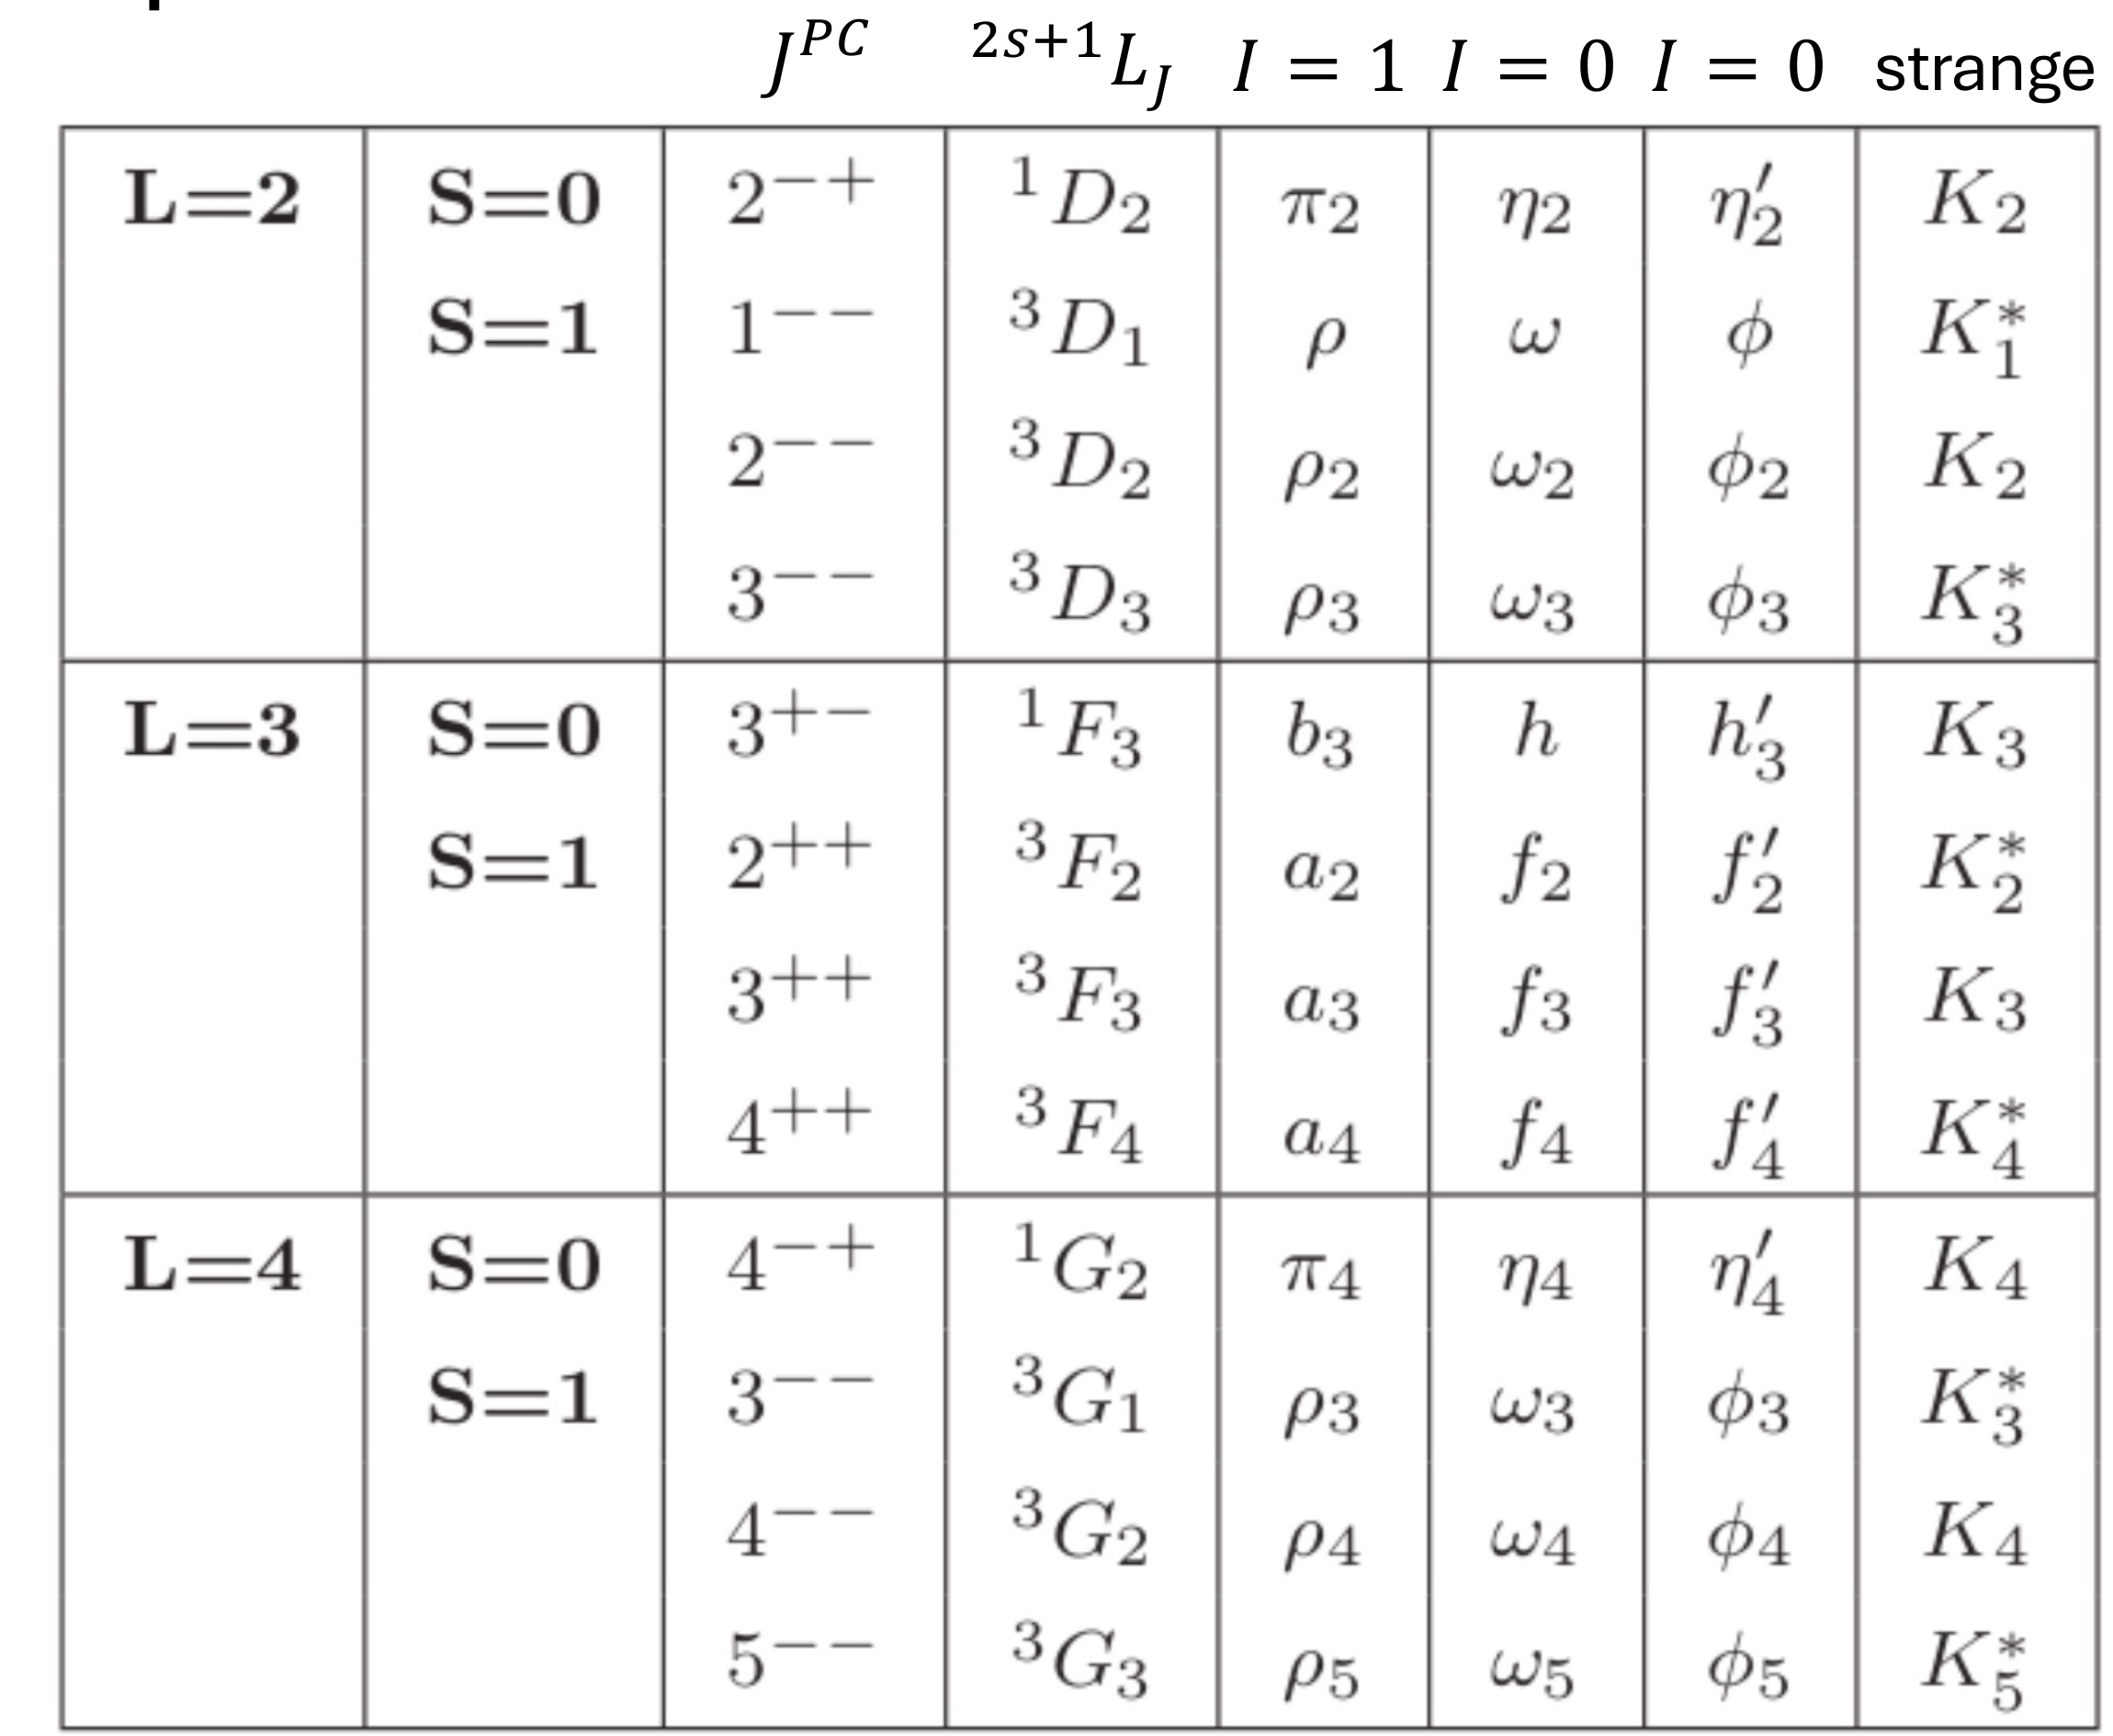
\includegraphics[width=0.65\linewidth]{Figures/meson_naming_extended.png}
    \caption{Continuation of the naming scheme for $L=2,3,4$ ($D$-, $F$- and
    $G$-wave mesons). Adapted from the lecture slides (week 19, "Conventional
    mesons: Naming scheme").}
    \label{fig:meson_naming_extended}
\end{figure}

% ============================================================
\subsection{The \texorpdfstring{$\eta$}{eta} meson as a gateway to QCD and new physics}
\label{subsec:eta-gateway}

The $\eta$ occupies a special place among the light mesons. With a mass of
$m(\eta) = 548$~MeV it has ample phase space to decay into pions, yet its quantum
numbers $I^{G}(J^{PC}) = 0^+ 0^{-+}$ forbid or suppress the most obvious channels,
turning the particle into a sensitive testing ground for the symmetries of the strong
interaction \cite[Ch.~3]{Amsler2018}. The two-pion mode is forbidden outright: with
$J_\eta = 0$ the pions must be in a relative $S$ wave, giving the pair the parity
$P(\pi\pi) = (-1)^L\,P(\pi)^2 = +1$, in conflict with the negative parity of the
$\eta$. The three-pion mode respects parity but violates $G$ parity, since
$G(\eta) = +1$ while $G(3\pi) = (-1)^3 = -1$; equivalently, three isospin-$1$ pions
cannot be coupled to the isospin-$0$ of the $\eta$ in a fully symmetric way, so the
decay is forbidden by isospin symmetry. Nevertheless it is observed with a sizeable
branching ratio, $BR(\eta\to3\pi)\approx 55\%$ \cite[Ch.~3]{Amsler2018}.

The resolution is that isospin is not an exact symmetry: because $m_u \neq m_d$, the
$\pi^0$ and the $\eta$ mix,
\begin{equation}
    \ket{\eta_{\text{phys}}} = \ket{\eta} - \epsilon\,\ket{\pi^0},
    \qquad
    \epsilon \sim (m_d - m_u),
    \label{eq:pi_eta_mixing}
\end{equation}
so that the physical $\eta$ decays ``through'' its small $\pi^0$ admixture. The rate
of $\eta\to3\pi$ is therefore directly sensitive to the light-quark mass difference,
making the $\eta$ a precision laboratory for one of the fundamental parameters of
QCD \cite[Ch.~3]{Amsler2018}.

The same suppression of conventional channels makes the $\eta$ attractive as a
window onto physics beyond the Standard Model. With many of its strong and
electromagnetic decays forbidden or strongly suppressed, the relative weight of any
rare or symmetry-violating mode is enhanced. The rare radiative decay
$\eta \to \pi\gamma\gamma$, in particular, can be used to search for light, weakly
coupled mediators over a broad mass range: a new boson produced in
$\eta \to B'\gamma \to \pi^0\gamma\gamma$ or a light scalar in
$\eta \to \pi^0 S \to \pi^0\gamma\gamma$ would appear as a peak in the
$\pi^0\gamma$ (or diphoton) invariant-mass spectrum on top of the Standard-Model
continuum.

\begin{figure}[htbp]
    \centering
    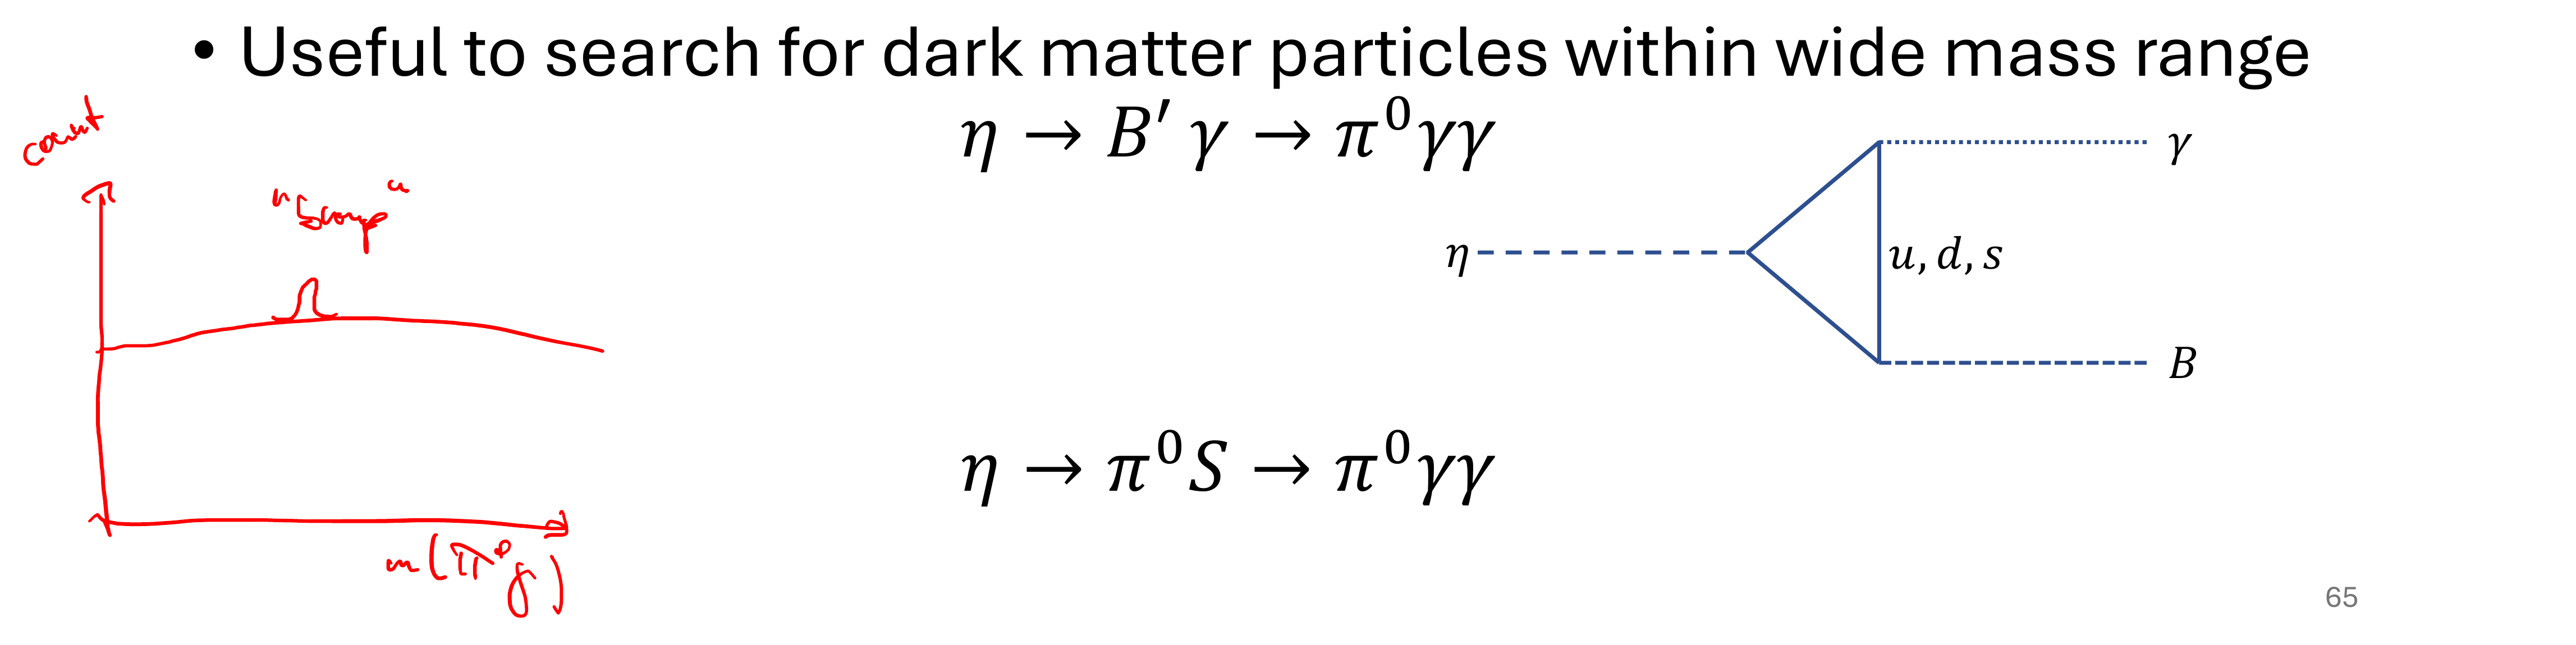
\includegraphics[width=0.85\linewidth]{Figures/eta_rare_decay.png}
    \caption{Quark-loop diagram for the rare decay
    $\eta\to\pi^0\gamma\gamma$ (via a $u,d,s$ triangle loop) and its
    new-physics variants $\eta\to B'\gamma\to\pi^0\gamma\gamma$ and
    $\eta\to\pi^0 S\to\pi^0\gamma\gamma$, together with a sketch of the
    expected $\pi^0\gamma$ invariant-mass spectrum: a hypothetical light
    mediator would appear as a narrow ``bump'' over the Standard-Model
    continuum. Adapted from the lecture slides (week 19, "The eta meson as
    gate to new physics").}
    \label{fig:eta_rare_decay}
\end{figure}